\section{Explaining the bandits' decisions}\label{sec:13}

\begin{figure}[!htbp]\centering
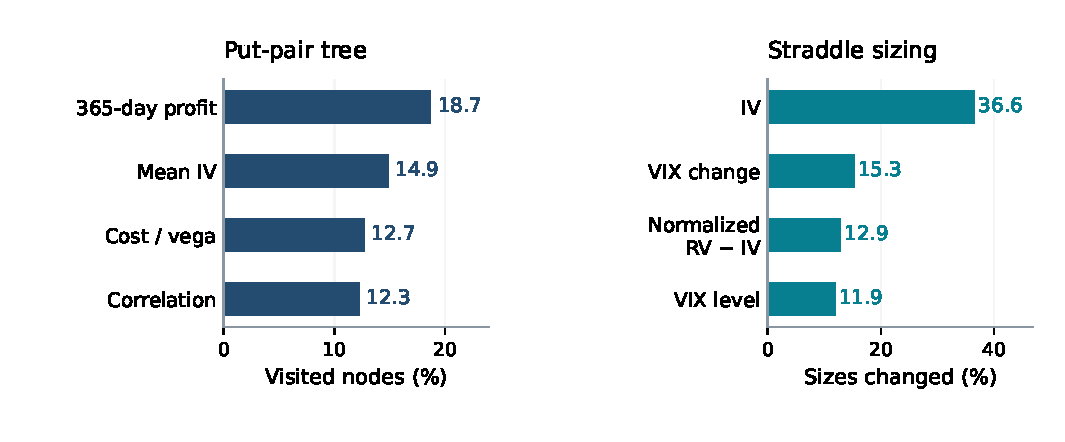
\includegraphics[width=\linewidth]{entry_explanations.pdf}
\caption{Put bars show the share of visited tree nodes; straddle bars show size changes when one input is centered. The denominators differ. Both are descriptive policy-usage measures.}\label{fig:entry-explanations}
\end{figure}

\subsection*{From an input to a requested trade size}

For a put proposal, interpretation is exact: follow the saved tree's root-to-leaf conditions, then read the size assigned to that leaf. Completed 365-day profitability appears in 18.7\% of later visited decision nodes, mean IV in 14.9\%, commission relative to vega in 12.7\%, and stock-return correlation in 12.3\%. These frequencies describe which information the fitted policy uses; they are not causal effects or a ranking of expected profit contributions.


For a straddle proposal, standardized ridge contributions add to a score. Saved thresholds locate its context, and the learned map selects a size. Centering IV changes 36.6\% of later fitted proposal sizes. Recent VIX change changes 15.3\%, normalized RV-minus-IV memory 12.9\%, and VIX level 11.9\%. The size map need not rise monotonically with the regression score because it optimizes the combined daily path. Exact replay reproduces every saved size across all 608 put and 35,774 straddle proposals.


\begin{center}\small
\setlength{\tabcolsep}{4pt}\renewcommand{\arraystretch}{1.18}
\begin{tabularx}{\textwidth}{@{}>{\hsize=1.89062\hsize\linewidth=\hsize\raggedright\arraybackslash}X>{\hsize=0.70312\hsize\linewidth=\hsize\raggedleft\arraybackslash}X>{\hsize=0.70312\hsize\linewidth=\hsize\raggedleft\arraybackslash}X>{\hsize=0.70312\hsize\linewidth=\hsize\raggedleft\arraybackslash}X@{}}\toprule
Later entry overlap vs full & Both & Bandit only & Fixed only\\\midrule
Put pairs & 74 & 36 & 1\\
Straddles & 897 & 307 & 43\\
\bottomrule\end{tabularx}\end{center}

Admission provides a second explanation for performance. Against fixed full size, the put bandit enters 36 later opportunities that the fixed policy rejects and misses one that it accepts. For straddles, those counts are 307 and 43. These differences can arise through the inventory left by earlier size decisions. An explanation of proposed size alone therefore does not explain the entire portfolio result.


Among quote-available completed straddle labels, full-size profit averages \$1,631 for proposals assigned full size and \$16 for those assigned half size. This subset is conditioned on available labels. Three within-date size shuffles yield later Sharpes 0.834, 0.928 and 1.044, versus 1.041 learned. One shuffle wins: favorable funded results and feature usage do not by themselves establish predictive sizing.


\FloatBarrier
